\documentclass{instrukcja}        
\usepackage[polish]{babel}
\usepackage[utf8]{inputenc}
\usepackage[OT4]{fontenc}

\begin{document}

\materialnumber{9}
\course[Info I]{Informatyka I}
\material[Lab 9]{Instrukcja 9}
\author{B. Górecki}
\materialtitle


\section{Oblężenie}
Do poprzednich zajęć poznaliśmy już wszystkie instrukcje zaplanowane na ten kurs języka C. Czas przejść do kilku nieco bardziej dojrzałych przykładów. Dziś zajmiemy się oblężeniem zamku. Twoim zadaniem jest napisać program, który będzie symulował ostrzał zamku przez kule armatnie (kule lecą wg wzorów na rzut ukośny). Program powinien kolejno:
\begin{itemize}
\item Przygotować okno graficzne o wymiarach 800 x 600.
\item Narysować zamek, który będziemy burzyć (kod funkcji rysującej zamek możesz znaleźć na końcu instrukcji).
\item W pętli:
\begin{itemize}
\item wczytywać z klawiatury wartość prędkości wylotowej kuli \begin{math} V_0 \end{math}, kąta odchylenia lufy od poziomu \begin{math} \alpha \end{math} oraz położenie armaty wzdłuż współrzędnej {\it x} (wylot armaty zawsze ma się znajdować 50 jednostek powyżej poziomu ziemi).
\item ustawiać i rysować schematycznie armatę jako jedną linię (należy przy tym sprawdzać, czy w danym miejscu da się postawić armatę - mur zamku znajduje się w obszarze \begin{math} x \geq 550 \end{math}; dla uproszczenia radzimy przy tym rysować armatę, jako linię o górnym wierzchołku w punkcie {\it (x, 50)} i dolnym wierzchołku zależnym od kąta wychylenia).
\item wykonywać strzał kulą i rysować jej tor za pomocą gęsto rozłożonych okręgów o małym promieniu - użyj funkcji {\tt animate} w celu uzyskania efektu płynnego ruchu kuli (przykład użycia funkcji {\tt animate} na końcu instrukcji). Tor rzutu ukośnego dany jest wzorami:
\begin{equation}
x(t) = x_0 + V_0 sin(\alpha)t
\end{equation}
\begin{equation}
y(t) = y_0 + V_0 cos(\alpha)t - \frac{gt^2}{2}.
\end{equation}
Program powinien cały czas w pętli sprawdzać, czy kula nie uderzyła w pierwszą, pionową ścianę zamku. Jeśli tak, kula ma się na niej zatrzymać, a pętla ulec przerwaniu. W przeciwnym razie program ma tak długo rysować ruch kuli, aż ta znajdzie się na ujemnych wartościach współrzędnej {\it y}. Ściana zamku zawiera się w przedziale \begin{math} 550 \leq x \leq 600 \end{math} oraz jej górna powierzchnia ma współrzędną \begin{math} y = 300 \end{math}.\\
Pamiętaj również o przeliczeniu współrzędnych fizycznych (pionowej) na współrzędną w układzie współrzędnych ekranu oraz przeliczeniu kąta podawanego w stopniach na kąt podany w radianach na potrzeby funkcji trygonometrycznych.
\item Po wykonanym strzale program zapyta, czy udało się trafić w zamek. Jeśli odpowiesz twierdząco, zakończy działanie programu. Jeśli przecząco, pozwoli wybrać nowe parametry strzału i będzie powtarzał tę operację aż do chwili uzyskania satysfakcjonującego cię wyniku.
\end{itemize}
\end {itemize}
\subsection*{Wskazówka}
W niniejszym programie w ogóle nie używaj funkcji {\tt wait()}. Program z wykonaniem i tak będzie czekać na podanie nowego zestawu danych do funkcji {\tt scanf()}.
\subsection*{Oczekiwany wynik}
Spodziewamy się, że wynikiem działania twojego programu będzie efekt zbliżony do tego pokazanego na Rysunku 1.
\begin{figure}
\centering
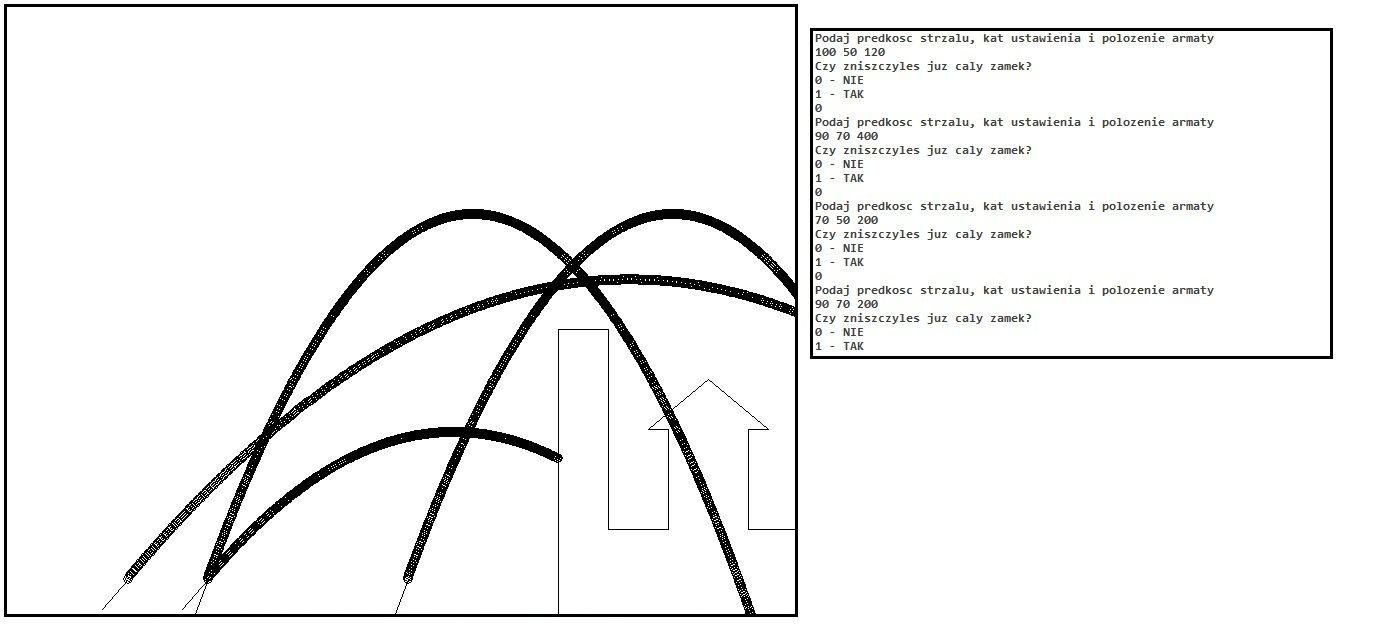
\includegraphics[width=0.45\textwidth]{zamek2.jpg}
\caption{Oczekiwany efekt działania programu}
\end{figure}
\subsection*{Dodatki}
Funkcja {\tt animate} tak naprawdę jedynie spowalnia wykonywanie pętli {\tt while} tak, aby kółka nie rysowały się zbyt szybko. Przykład jej użycia wygląda następująco:
\begin{verbatim}
while(animate(100)) // Wartosc 0 oznacza najszybsze mozliwe
                    // wykonanie (brak opoznienia)
{
   // Oblicz tu nowe wspolrzedne x i y
   // Narysuj okrag w odpowiednim miejscu
   // Zwieksz parametr t
   // Zawrzyj warunek przerwania petli, gdy kula uderza
   // w sciane lub spada na y < 0
}

void RysujZamek()
{
   line(550, 300, 550, 600);
   line(550, 300, 600, 300);
   line(600, 300, 600, 500);
   line(600, 500, 660, 500);
   line(660, 500, 660, 400);
   line(660, 400, 640, 400);
   line(640, 400, 700, 350);
   line(700, 350, 760, 400);
   line(760, 400, 740, 400);
   line(740, 400, 740, 500);
   line(740, 500, 800, 500);
}
\end{verbatim}

\end{document}
